\section{Chapter 3}
\subsection{Exercises}

\begin{sol}{Exercise 3.1}
Try some of your own polynomials. Start with polynomials of the form
\[
ax^2 + bx + c
\]
and work your way up higher-degree polynomials. For example, have you tried the polynomial
\[
x^2 -x - 1
\]
Try some more of your own. Vieta's formulas should be working!
\end{sol}

\begin{sol}{Exercise 3.2}
I will show the backwards proof of AM-GM, working from the AM-GM inequality and manipulating it into a known fact.
\[
\frac{a+b}{2} \geq \sqrt{ab}
\]
\[
a+b \geq 2\sqrt{ab}
\]
\[
a^2 + b^2 + 2ab \geq 4ab
\]
\[
a^2 + b^2 - 2ab \geq 0
\]
\[
(a-b)^2 \geq 0
\]
which is known as the trivial inequality, since
\[
\forall x \in \mathbb{R}, x^2 \geq 0
\]
and is trivially true. We got our proof by simply doing these steps in reverse, and perhaps this shows some motivation behind some steps in the original proof.
\end{sol}

\begin{sol}{Exercise 3.3}
This is another example of direct proof.
\begin{proof}
If n is odd, then $\exists k \in \mathbb{Z}$ such that $n = 2k + 1$. We then substitute this
\[
(2k+1)^2 + (2k+1) = 4k^2 + 4k + 1 + 2k + 1 = 4k^2 + 6k + 2
\]
\[
= 2(2k^2 + 3k + 1)
\]
which is clearly even.
\end{proof}
\end{sol}

\begin{sol}{Exercise 3.4}
Read the following text, until the tree diagram to understand the breakdown of cases. We will be referring to the tree diagram to break up the problem into cases and calculate the final result.
\begin{center}
\scalebox{0.65}{
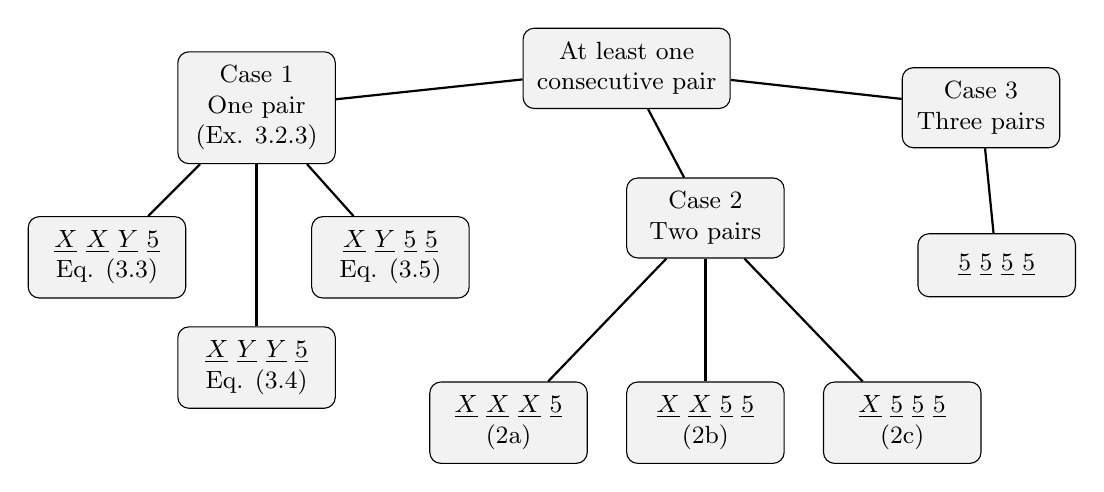
\begin{tikzpicture}[
  every node/.style={font=\small, align=center},
  box/.style={draw, rounded corners, fill=gray!10, inner sep=5pt, minimum width=2cm, minimum height=0.8cm},
  line/.style={draw, thick}
]

% Root node
\node[box] (root) at (0, 0) {At least one\\consecutive pair};

% Level 1 nodes
\node[box] (c1) at (-4.7, -.5) {Case 1\\One pair \\(Ex. 3.2.3)};
\node[box] (c2) at (1, -1.9) {Case 2\\Two pairs};
\node[box] (c3) at (4.5, -0.5) {Case 3\\Three pairs};

% Level 2 nodes - Case 1 children
\node[box] (c1a) at (-6.6, -2.4) {$\underline{X}~\underline{X}~\underline{Y}~\underline{5}$\\Eq. (3.3)};
\node[box] (c1b) at (-4.7, -3.8) {$\underline{X}~\underline{Y}~\underline{Y}~\underline{5}$\\Eq. (3.4)};
\node[box] (c1c) at (-3, -2.4) {$\underline{X}~\underline{Y}~\underline{5}~\underline{5}$\\Eq. (3.5)};

% Level 2 nodes - Case 2 children
\node[box] (c2a) at (-1.5, -4.5) {$\underline{X}~\underline{X}~\underline{X}~\underline{5}$\\(2a)};
\node[box] (c2b) at (1, -4.5) {$\underline{X}~\underline{X}~\underline{5}~\underline{5}$\\(2b)};
\node[box] (c2c) at (3.5, -4.5) {$\underline{X}~\underline{5}~\underline{5}~\underline{5}$\\(2c)};

% Level 2 nodes - Case 3 child
\node[box] (c3a) at (4.7, -2.5) {$\underline{5}~\underline{5}~\underline{5}~\underline{5}$};

% Lines from root to level 1
\draw[line] (root) -- (c1);
\draw[line] (root) -- (c2);
\draw[line] (root) -- (c3);

% Lines from Case 1 to its children
\draw[line] (c1) -- (c1a);
\draw[line] (c1) -- (c1b);
\draw[line] (c1) -- (c1c);

% Lines from Case 2 to its children
\draw[line] (c2) -- (c2a);
\draw[line] (c2) -- (c2b);
\draw[line] (c2) -- (c2c);

% Lines from Case 3 to its child
\draw[line] (c3) -- (c3a);

\end{tikzpicture}
}
\end{center}
We have already counted case 1 in Example 3.9, which gave us 168 numbers. Thus, all that remains is case 2 and 3. 

We will begin with case 2. Starting with case (2a), we know that $X$ may be any of the 8 digits not equal to $0$ or $5$ (if $X = 5$, then we are at case 3). Thus, we have 8 different numbers that are in this case. Case (2b) gives us something very similar, as there are still 8 options, and again there are 8 option for $X$ in case (2c) as well. Summing up all the numbers that satisfy case 2:
\[
\overbrace{8}^{(2a)} + \overbrace{8}^{(2b)} + \overbrace{8}^{(2c)} = 24
\]

Now, we move on to case 3. $5555$ is the only number that satisfies case 3, so we simply add $1$.

Therefore, the final answer is the sum of each case, which is
\[
\overbrace{168}^{\text{Case 1}} + \overbrace{24}^{\text{Case 2}} + \overbrace{1}^{\text{Case 3}} = \boxed{193}
\]
\end{sol}


\subsection{Problems} % Chapter 3
\begin{sol}{Problem 3.1}
\begin{proof}
$n^2 + n$ factors into $n(n+1)$. If $n$ is even, then the expression is trivially even. If $n$ is odd, then $n+1$ is even and so the expression is still even. Therefore, $n(n+1)$ must always be even, and since $n(n+1) = n^2 + n$, we have proved $n^2 + n$ must always be even.
\end{proof}
\end{sol}

\begin{sol}{Problem 3.2}
\begin{proof}
By definition, since we are working only in positive integers (else $b$ could be negative, which complicates things...)
\[
a \mid b \implies a \leq b
\]
Similarly,
\[
b \mid a \implies b \leq a
\]
Since $b \leq a$ and $a \leq b$, the only such $a$ and $b$ that satisfy this are such that
\[
a = b
\]
\end{proof}
\end{sol}

\begin{sol}{Problem 3.3}
This problem does not explicitly ask for a proof, and rather tests your ability to use casework. I will present a "proof" which is essentially a walkthrough of the solution.
\begin{proof}
There are three cases, of which we obtain endpoints from when the argument of each absolute value function changes sign. 
\begin{enumerate}
    \item $x \leq -2$
    \item $-2 < x \leq 1$
    \item $1 < x$
\end{enumerate}
Beginning with case 1, if $x \leq -2$, we have that $x + 2 \leq 0$. If $x \leq -2$, then $x - 1 < 0$. Thus, since the absolute value always returns the positive, we negate both arguments of absolute values. If $x \leq 2$, then 
\[
|x + 2| + |x-1| = -(x+2) -(x-1) = -2x -1
\]
and so we search for the set 
\[
\{x : x \leq -2\} \cap\{x : -2x-1 \leq 4 \}
\]
simplifying, we get 
\[
-2x-1 \leq 4
\]
\[
-2x \leq 5
\]
\[
x \geq -\frac{5}{2}
\]
and so solutions occur when 
\[
\{x : x \leq -2\} \cap\{x : x \geq -\frac{5}{2} \}
\]
which is the closed interval $\left[-\frac{5}{2}, -2\right]$.

Next, for case 2, $-2 < x \leq 1$. This implies that $x + 2 > 0$ and $x - 1 \leq 0$. Thus, we only negate the $x - 1$ term to "carry through" the absolute value.
\[
|x + 2| + |x-1| = x + 2 -(x-1) = 3
\]
which is always less than 4. Therefore, we also have the set of solutions where $-2 < x \leq 1$ which is the interval $(-2, 1]$.

Finally, case 2, $1 < x$. This implies $x + 2 > 0$ and $x - 1 > 0$, so we simplify the absolute values to become
\[
|x + 2| + |x-1|  = x + 2 + x - 1 = 2x + 1
\]
and we are looking for the set
\[
\{x : x > 1\} \cap\{x : 2x+1 \leq 4 \}
\]
which when simplified, is 
\[
\{x : x > 1\} \cap\{x :  x \leq \frac{3}{2}\}
\]
which is the interval $\left(1, \frac{3}{2}\right]$. 

To combine the cases, we seek the union of these intervals
\[
\left[-\frac{5}{2}, -2\right] \cup (-2, 1] \cup \left(1, \frac{3}{2}\right]
\]
which evaluates to the closed interval
\[
\boxed{\left[-\frac{5}{2}, \frac{3}{2}\right]}
\]
\end{proof}
\end{sol}

\begin{sol}{Problem 3.4}
\begin{proof}
We will begin with the forwards direction, proving that 
\[
p \mid a \implies p \mid a^2
\]
We simply apply the fact (which is also logically deducible) that if $k \mid m$, then $k \mid m \cdot a$ for all integers $a$. since $p \mid a$, we have that $p \mid a \cdot a$, which proves the forwards direction. 

Now, for the backwards direction, we want to prove
\[
p \mid a^2 \implies p \mid a
\]
we use a fact known as Euclid's Lemma. Euclid's lemma states that if we have, for prime $p$, that $p \mid ab$, then either $p \mid a$ or $p \mid b$. In this case, we apply this to the fact that 
\[
p \mid a^2 \implies p \mid a \cdot a \implies (p \mid a \text{ or } p \mid a)
\]
which gives is that $p \mid a$. Therefore, we have proved both sides of the statement.
\end{proof}

For those not satisfied with Euclid's Lemma, try playing around with it yourself. Figure out why $p$ must be prime for Euclid's Lemma to work. Even if you do not know Euclid's lemma by name, it is a property you might be able to infer from numbers. 
\end{sol}

\begin{sol}{Problem 3.5}
\begin{proof}
This is false in general. We can see this when we expand
\[
(a + b)^2 = a^2 + b^2 + 2ab
\]
which is only equal to $a^2 + b^2$ when $2ab$ is zero. Thus, for any $a, b$ such that $ab \neq 0$, we have that the statement is false. More concretely, for example, $a = 1, b = 2$ clearly fails the test, since $(1 + 2)^2 = 9$ while $1^2 + 2^2 = 5$. 

However, this discussion has led us to find when exactly these are the same.
\[
(a + b)^2 = a^2 + b^2 + 2ab = a^2 + b^2
\]
after subtracting $a^2 + b^2$ from both sides,
\[
2ab = 0
\]
So when either $a$ or $b$ (or both) equal 0, we have that this equation does hold (trivially, since we them just get, for $a = 0$, $(b)^2 = b^2$).
\end{proof}
\end{sol}

\begin{sol}{Problem 3.6}
\begin{proof}
We begin by factoring the left-hand side
\[
x^2 + 3x \equiv x(x+3) \equiv 0 \pmod{5}
\]
which is simply a quadratic equation. The two possible solutions occur when either 
\[
x \equiv 0 \pmod{5} ~\text{  or  } ~x + 3 \equiv 0 \pmod{5}
\]
and simplifying the latter gives us
\[
x \equiv 2 \pmod{5}
\]
Therefore, all integers congruent to either 
\[
\boxed{0 \text{ or } 2 \pmod{5}}
\]
satisfy the equation.
\end{proof}
Note that we have to be careful. We are allowed to assume either $x \equiv 0 \pmod{5}$ or $x + 3 \equiv 0 \pmod{5}$ because $5$ is prime. For example, consider a non-prime number, say 6. If we have that $xy \equiv 0 \pmod{6}$, we cannot simply assume, that $x$ or $y$ is congruent to 0 $\pmod{6}$, since that leaves out the case, for example, when $x \equiv 2 \pmod{6}$ and $y \equiv 3 \pmod{6}$, or vice versa. Since $5$ is prime, we do not have to worry about these other cases, since the only such numbers that multiply to 5 are $1 \times 5$, and $5 \equiv 0 \pmod{5}$. The primality of 5 makes the solution more simple, but always keep in mind to check for these traps!
\end{sol}

\begin{sol}{Problem 3.7}
\begin{proof}
We apply the AM-GM inequality to positive real numbers $a$ and $\frac{1}{a}$
\[
\frac{a + \frac{1}{a}}{2} \geq \sqrt{a \cdot \frac{1}{a}}
\]
\[
a + \frac{1}{a} \geq 2 \cdot \sqrt{1}
\]
\[
a + \frac{1}{a} \geq 2
\]
\end{proof}
This relatively simple example probably does not benefit from working backwards, from starting with $a + \frac{1}{a} \geq 2$ and manipulating it into a known quantity because it is hard to see the steps of adding a $\cdot \sqrt{1}$ and expanding $1$ into $a \cdot \frac{1}{a}$. However, once you know that you need to use AM-GM, it is typically not too hard to see that a simple application gives us the result we need.
\end{sol}

\begin{sol}{Problem 3.8}
This is a bit of a difficult problem, inspired by math olympiad problems. This takes significant ingenuity, so don't be discouraged if you did not get this!
\begin{proof}
We first present and prove a couple lemmas (not common) used in the main proof.

\textbf{Lemma P3.8.1}
\[
ab + bc + ca = \frac{1 - (a^2 + b^2 + c^2)}{2}
\]
\begin{proof}
We prove lemma P3.8.1. We know that 
\[
a + b + c = 1
\]
and thus we can square both sides to obtain
\[
(a+b+c)^2 = 1
\]
\[
a^2 + b^2 + c^2 + 2(ab + bc + ca) = 1
\]
which we then rearrange 
\[
2(ab + bc + ca) = 1 - (a^2 + b^2 + c^2)
\]
\[
ab + bc + ca = \frac{1 - (a^2 + b^2 + c^2)}{2}
\]
\end{proof}

\textbf{Lemma P3.8.2}
\begin{proof}
We prove lemma P3.8.2. 
By the AM-GM inequality on each pair of integers squared, we have 
\[
\begin{cases}
\frac{a^2 + b^2}{2} \geq \sqrt{a^2b^2} \\
\frac{b^2 + c^2}{2} \geq \sqrt{b^2c^2} \\
\frac{c^2 + a^2}{2} \geq \sqrt{c^2a^2}
\end{cases}
\]
which simplify to
\[
\begin{cases}
\frac{a^2 + b^2}{2} \geq ab \\
\frac{b^2 + c^2}{2} \geq bc \\
\frac{c^2 + a^2}{2} \geq ca
\end{cases}
\]
and when we sum each of the three equations, we get
\[
a^2 + b^2 + c^2 \geq ab + bc + ca
\]
\end{proof}
Since by Lemma P3.8.1
\[
ab + bc + ca = \frac{1 - (a^2 + b^2 + c^2)}{2}
\]
we substitute this equality into the inequality obtained in Lemma P3.8.2
\[
a^2 + b^2 + c^2 \geq \frac{1 - (a^2 + b^2 + c^2)}{2}
\]
which we rearrange and solve
\[
2(a^2 + b^2 + c^2) \geq 1 - (a^2 + b^2 + c^2)
\]
\[
3(a^2 + b^2 + c^2) \geq 1
\]
\[
a^2 + b^2 + c^2 \geq \frac{1}{3}
\]
This implies that 
\[
1 - (a^2 + b^2 + c^2) \leq \frac{2}{3}
\]
which implies that
\[
\frac{1 - (a^2 + b^2 + c^2)}{2} \leq \frac{1}{3}
\]
and substituting using Lemma P3.8.1, we get
\[
ab + bc + ca \leq \frac{1}{3}
\]
End of proof of Problem 3.8.
\end{proof}

It is often difficult to find the exact motivation and reasoning behind why we chose to do certain steps. This is exactly why olympiad mathematics (which this problem tried to emulate at a simpler scale) is so difficult! Once you see the solution, it often feels obvious, or very easy, but "seeing" the solution on your own is usually the hard part.
\end{sol}

\begin{sol}{Problem 3.9}
\begin{proof}
\[
a \equiv b \pmod{7} \implies a - b \equiv 0 \pmod{7}
\]
which implies
\[
7 \mid (a - b)
\]
Since $P(x)$ is a polynomial with integer coefficients, we simply apply the "polynomial division theorem" (Theorem 3.3).
\[
a - b \mid P(a) - P(b)
\]
and since $7 \mid (a-b)$, we have that (by transitive property, is $a \mid b$ and $b \mid c$, then $a \mid c$)
\[
7 \mid P(a) - P(b)
\]
\end{proof}
\end{sol}

\begin{sol}{Problem 3.10}
For a polynomial of the form 
\[
ax^3 + bx^2 + cx + d
\]
Vieta's formulas say that
\[
\begin{cases}
r_1 + r_2 + r_3 = -\frac{b}{a} \\
r_1r_2 + r_2r_3 + r_3r_1 = \frac{c}{a} \\
r_1r_2r_3 = -\frac{d}{a}
\end{cases}
\]
so for part (a), we get that the answer is simply
\[
-\frac{-3}{2} = \boxed{\frac{3}{2}}
\]
and for part (b), it is
\[
\boxed{\frac{1}{2}}
\]
For part (c), we need a little more thinking. Expanding $(r_1 + r_2 + r_3)^2$ gives us
\[
(r_1 + r_2 + r_3)^2 = r_1^2 + r_2^2 + r_3^2 + 2(r_1r_2 + r_2r_3 + r_3r_1)
\]
which we rearrange to isolate the term we are interested in
\[
r_1^2 + r_2^2 + r_3^2 = (r_1 + r_2 + r_3)^2 - 2(r_1r_2 + r_2r_3 + r_3r_1)
\]
and since we know the values of the terms on the right hand side (we just calculated them), we can simply substitute
\[
r_1^2 + r_2^2 + r_3^2 = \left(\frac{3}{2}\right)^2 - 2 \cdot \left(\frac{1}{2}\right) 
\]
\[
= \frac{9}{4} - 1  = \boxed{\frac{5}{4}}
\]
\end{sol}

\begin{sol}{Problem 3.11}
This is yet again another difficult problem which uses Vieta's formulas as a key step, in which there are many other manipulations to be made. Again, do not be discouraged if you are looking at the solutions as a last resort; this is a difficult probem.
\begin{proof}
WLOG, number the roots $r_1, r_2, \ldots, r_{4050}$ such that the polynomial $x^2 - 4x - 3$ has roots $r_1, r_2$, the polynomial $2x^2 - 4x - 3$ has roots $r_3, r_4$ and the polynomial $kx^2 - 4x - 4$ has roots $r_{2k-1}, r_{2k}$. The harmonic mean of all these roots is 
\[
\frac{1}{\frac{1}{4050}\left( \frac{1}{r_1} + \frac{1}{r_2} + \frac{1}{r_3} + \frac{1}{r_4} + \cdots \frac{1}{r_{4049}} + \frac{1}{r_{4050}} \right)}
\]
We want to evaluate this. To begin, we will try to evaluate the expression
\[
\left( \frac{1}{r_1} + \frac{1}{r_2} + \frac{1}{r_3} + \frac{1}{r_4} + \cdots \frac{1}{r_{4049}} + \frac{1}{r_{4050}} \right)
\]
We group these roots by two, such that each group is from the same underlying polynomial. 
\[
\left( \underbrace{\frac{1}{r_1} + \frac{1}{r_2}}_{k = 1} + \underbrace{\frac{1}{r_3} + \frac{1}{r_4}}_{k = 2} + \cdots \underbrace{\frac{1}{r_{4049}} + \frac{1}{r_{4050}}}_{k = 2025} \right)
\]
For a general grouping
\[
\underbrace{\frac{1}{r_{2k-1}} + \frac{1}{r_{2k}}}_{k}
\]
from polynomial $kx^2 - 4x - 3$, we can simplify the expression. 
\[
\frac{1}{r_{2k-1}} + \frac{1}{r_{2k}} = \frac{r_{2k} + r_{2k-1}}{r_{2k-1}r_{2k}}
\]
now, we use Vieta's theorems to obtain
\[
\begin{cases}
r_{2k} + r_{2k-1} = \frac{4}{k} \\
r_{2k-1}r_{2k} = \frac{-3}{k}
\end{cases}
\]
which we substitute into the general grouping expression to obtain 
\[
\frac{r_{2k} + r_{2k-1}}{r_{2k-1}r_{2k}} = \frac{\frac{4}{k}}{-\frac{3}{k}} = -\frac{4}{3}
\]
and thus every grouping always evaluated to $-\frac{4}{3}$. Since there are 2025 such groups of two from 2025 polynomials, we have that 
\[
\frac{1}{\frac{1}{4050}\left( \frac{1}{r_1} + \frac{1}{r_2} + \frac{1}{r_3} + \frac{1}{r_4} + \cdots \frac{1}{r_{4049}} + \frac{1}{r_{4050}} \right)} 
\]
\[
= \frac{1}{\frac{1}{4050}\left(2025 \cdot -\frac{4}{3} \right)}
\]
\[
= \frac{1}{\frac{1}{2}\cdot -\frac{4}{3}} = \frac{1}{-\frac{2}{3}} = \boxed{-\frac{3}{2}}
\]
\end{proof}
\end{sol}

\begin{sol}{Problem 3.12}
\begin{proof}
We split this into 3 cases. First, when $n = 1$, second, when $n$  is odd but $> 1$ and third, when $n$ is even. Next, let $f(n) := 2^n + 12^n + 2011^n$
We will consider residues modulo 4. If a number is a perfect square, it must be congruent to either $0$ or $1$ $\pmod{4}$. First, let us simplify $f(n)$ $\pmod{4}$. 
\[
f(n) \equiv 2^n + 0^n + 3^n \equiv 2^n + (-1)^n\pmod{4}
\]
When $n = 1$, we get that this simplifies to 
\[
f(n) \equiv 1 \pmod{4}
\]
and thus we plug in $n=1$ to see if we get a perfect square. $f(1) = 2025 = 45^2$, so $n=1$ is a solution. 

Now, we consider odd $n$ which is greater than 1. Note that for all $n \geq 2$, $2^n \equiv 0 \pmod{4}$. This allows us to simplify, given the assumption that $n$ is odd and $\neq 1$,
\[
f(n) \equiv 0 + -1 \equiv -1 \pmod{4}
\]
which shows that there are no solutions that are perfect squares when n is odd and greater than 1, because perfect squares are always 0 or 1 $\pmod{4}$. 

Next, consider even $n$. This time, we will consider residues $\pmod{3}$, with the same restriction that perfect squares must be either $0$ or 1 $\pmod{3}$.
\[
f(n) \equiv (-1)^n + 1^n \pmod{3}
\]
and for even $n$, we have that
\[
f(n) \equiv 1 + 1 \equiv 2 \pmod{3}
\]
and since it is not congruent to 0 or 1, we have that there are no perfect squares when n is even.

Therefore, the only solution is $\boxed{n=1}$, which gives $f(1) = 2025 = 45^2$.
\end{proof}

The known facts that perfect squares are either congruent to o or 1 $\pmod{3}$ and $\pmod{4}$ were the key facts that helped us solve this problem. Again, as with olympiad problems, the most difficult aspect is learning the reasoning and motivation behind why we decided to choose this approach. In full honesty, the way I discovered the mod approach was by rote trial and error, as typically taking mods of complicated equations both simplify them and the perfect square allows us to get better numerical constraints. The parity case-split arose from considering the $(-1)^n$, which changes value based on parity. Further, the case-split $n=1$ arose due to the fact that $2^n \equiv 0 \pmod{4}$ for all $n > 1$. After playing around with the problem and identifying these facts, this slowly led to a complete solution. However, there are other ways to think about this and do it, and finding an approach that works is usually always the hardest part!
\end{sol}